\documentclass[main.tex]{subfiles}
\begin{document}
\newpage
\section{ Лекция 3. Продолжение описания ЛНСАУ }

12 февраля 2021 г.

\[ \xrightarrow{u}\boxed{\text{ОУ}}\xrightarrow{y} \]

Мы разобрали первый вид описания -- с помощью ДУ (он же \emph{операторный} вид описания, он же <<вход-выход>>):

\[ \alpha(D)y = \beta(D)U \thickspace + \text{ н. у. } \]

\subsection{Описание с помощью операторной передаточной функции}

В первом выражении разделим на $ \alpha(D) $; обозначим $ H(D) := \frac{\alpha(D)}{\beta(D)} $ -- \emph{операторная передаточная функция} (ОПФ).

У нас будет несколько передаточных функций; это -- операторная, т. к. зависит от оператора дифференцирования.

Теперь можем записать так:

\[ \xrightarrow{u}\boxed{H}\xrightarrow{y} \]

Единственная неприятность: пусть, к примеру, $ \beta(D) = (D - a), \alpha(D) = (D-a)(D-b) $.
При этом нельзя сократить на $ (D - a) $, т. к. можем сократить неустойчивость (если $ a > 0 $).

\subsubsection{Преобразование Лапласа}

$$ \mathds{L}\{f(t)\} = \bar{f}(p) = \int_0^{+\infty} e^{-pt} f(t) dt $$

Для чего переходим от вещественных функций к комплексным?
Дифференциальные уравнения (а также интегральные и интегро-дифференциальные) в изображениях сводятся к линейным алгебраическим уравнениям.
Это достигается за счёт свойства преобразования производной:

$$ \mathds{L}\{\dot f (t)\} = p \bar{f}(p)- f(0) $$

Устойчивые системы со временем <<забывают>> начальные условия, поэтому частая ситуация -- н. у. $= 0$.
Тогда $ \mathds{L}\{ f^{(n)}(t) \} = p^n \cdot \bar f(p) $ и уравнение \eqref{eq:linear_de} трансформируется так:
\[ \alpha(D)y = \beta(D)u \to \alpha(p) \cdot \bar y(p) = \beta(p) \cdot \bar u(p) \]

После преобразования уже ставится <<честный>> знак умножения $ \cdot $.

\[ \bar y(p) = \frac{\beta(p)}{\alpha(p)} \cdot \bar u(p) \]

\begin{equation}\label{eq:transmit_func}
    \boxed{\bar{y}(p) = H(p) \cdot \bar{u}(p) }
\end{equation}

$ H(p) $ -- \emph{ комплексная передаточная функция }.

Итак, у нас появились два варианта записи:

$$ \xrightarrow{u(t)} \boxed{H(D)}\xrightarrow{y(t)} $$

(вход -- функция времени, выход -- функция времени, произвольные постоянные н. у).

$$ \xrightarrow{\bar u(t)} \boxed{H(D)} \xrightarrow{ \bar y(t)} $$

(вход -- изображение, выход -- изображение, нулевые н. у).

\subsubsection{Преобразования некоторых функций}

\begin{enumerate}[noitemsep]
    \item Функция Хевисайда:
    \[ \mathds{L} \{ 1[t] \} = \frac{1}{p} \]
    \item Полином:
    \[ \mathds{L}\{ t^n \} = \frac{n!}{p^{n+1}} \]
    \item Тригонометрические функции:
    \[ \mathds{L}\{ \sin \omega t \} = \frac{\omega}{p^2 + \omega^2} \]
    \[ \mathds{L}\{ \cos \omega t \} = \frac{p}{p^2 + \omega^2} \]

\end{enumerate}

$ (\bar{\sin(t)})^2 + (\bar{\cos(t)})^2 \ne 1 $ (преобразование Лапласа линейное, а тригонометрические функции нелинейные).

\subsubsection{ Теорема затухания, пределы, преобразование от свёртки }

\[ \mathds{L}\{ f(t)e^{- \alpha t} \} = \bar f(p+\alpha) \]
откуда
\[ \mathds{L}\{ e^{- \alpha t} \} = \frac{1}{p+\alpha} \]

Часто требуется найти $ y_\infty $ и $ y(+0) $.

\[ y_\infty = \lim_{p \to 0} p \bar y(p) \]
\[ y(+0) = \lim_{p \to \infty} p \bar y(p) \]

Можно запомнить эти формулы по размерности.
Размерность аргумента преобразования Лапласа -- $ \frac{1}{\text{сек}} $ (экспоненту можно брать только от безразмерной величины).

Теорема о свёртке:
\[ \mathds{L}\{ \int_{0}^{t} f_1(\tau) f_2(t-\tau) d\tau  \} = \mathds{L}\{ \int_{0}^{t} f_1(t-\tau) f_2(\tau) d\tau \} = \bar f_1 (p) \cdot \bar f_2 (p) = \]

Ещё одно полезное преобразование:

\[ \mathds{L}\{ \sin (\omega t) e^{-\alpha t} \} = \frac{\omega}{(p + \alpha)^2 + \omega^2} \]

\subsection{Реализуемость}

Напомним, $ \alpha(D)y = \beta(D) u $, порядок $ \alpha $ -- $ n $, порядок $ \beta $ -- $ m $; $ n < m \Rightarrow $ нереализуемая система, $ n > m \Rightarrow $ строго реализуемая, $ n = m \Rightarrow $ нестрого реализуемая.

Покажем это, используя преобразование Лапласа.
Пусть вход системы -- функция Хевисайда.
\[ \xrightarrow{u = 1[t]}\boxed{H}\xrightarrow{y} \]

$$ \bar y = H(p) \bar u = \frac{\beta(p)}{\alpha(p)} \cdot \frac{1}{p} $$
\[ y(+0) = \lim_{p \to \infty} p \cdot \bar y = \lim_{p \to \infty} \frac{\beta(p)}{\alpha(p)} \]

При ограниченном входе, конечно же, должен быть ограниченный выход.
Значит, порядок знаменателя должен быть больше или равен порядку числителя, иначе получается бесконечность!

Скорость также не может меняться резко, скачком.
Поэтому, если $ y(t) = 0 $ при $ t < 0 $, то $ y(+0) = 0 $ тоже.
Это достигается только при $ n > m $ (строгая реализуемость).

\subsection{Третий способ описания: интегральное описание (описание при помощи весовой функции)}

\subsubsection{ Дельта-функция Дирака }

$$ \delta(t) = \begin{cases}
	0, t \ne 0 \\
	\infty, t = 0
 \end{cases} $$
+ условие нормировки: $ \int_{- \infty}^{+ \infty} \delta(t) dt $

(бесконечно узкий и бесконечно высокий импульс, площадь которого равна единице).

\textbf{Свойства:}
их можно доказать из предельного представления.
Введём функцию $ \tilde \delta (t) $ -- узкую и высокую ступеньку:

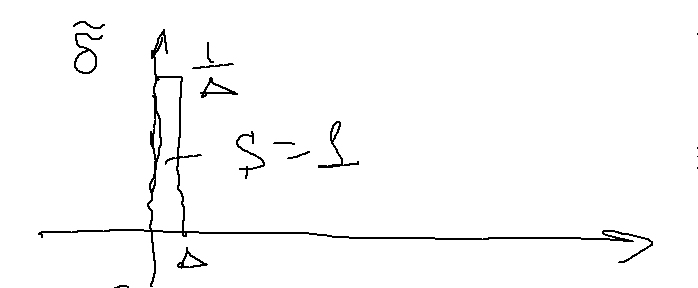
\includegraphics[width=.4\linewidth]{lec3/01_delta}

\[ \delta(t) = \lim_{\Delta \to 0} \tilde \delta(t) \]


\begin{enumerate}[noitemsep]
	\item Дельта-функция есть производная от функции Хевисайда.
	\item Фильтрующее свойство:
    пусть $ f(t) $ непрерывна в окрестности $ t_0 $.
    Тогда
    \[ \int_{-\infty}^{\infty} f(t) \delta(t-t_0) dt = f(t_0)  \]
    Для производной:
    \[ \int_{-\infty}^{\infty} f(t) \delta^{(n)}(t-t_0) dt = (-1)^n f^{(n)}(t_0) \]
\end{enumerate}

\subsubsection{ Интегральное описание }

Определение: \emph{ весовая функция }

\begin{equation} \label{eq:weight_fun}
    h(t) := \mathds{L}^{-1}\{ H(p) \}
\end{equation}

Введём новую функцию $ f(t) $:

$$ f(t) = \int_0^t h(t - \tau) u(\tau) d \tau $$

тогда
\[ \mathds{L}\{ f(t) \} = \bar h(p) \cdot \bar u(p) \overset{\eqref{eq:weight_fun}}= H(p) \cdot \bar u(p) \overset{\eqref{eq:transmit_func}}= \bar y(p) \]
\[ \mathds{L}\{ f(t) \} = \bar y(p) \Leftrightarrow f(t) \equiv y(t) \]

\begin{equation}\label{eq:third_form}
    content...
\end{equation}
$$ y(t) = \int_{0}^{t}h(t - \tau)u(\tau) d\tau = \int_{0}^{t}h(\tau)u(t - \tau) d\tau $$

Это -- третий вид описания!

Естественно, мы предполагаем, что н. у. $ =0 $ (ведь мы используем передаточую функцию; к тому же, $ y(0) = 0 $, как видно из интеграла).

Вторая форма удобна, если $ u = 1 $; третья, интегральная -- когда $ h $ есть простая функция.

\subsubsection{Физический смысл h(t). Переходная функция}

Найдём реакцию произвольной динамической системы, если на входе дельта-функция Дирака (и нулевые начальные условия).

\[ \xrightarrow{u(t)=\delta(t)}\boxed{H(D)}\xrightarrow{y(t) = ?} \]

Воспользуемся третим способом описания.

$$ y(t) \overset{\eqref{eq:third_form}}= \int_0^t h(t-\tau)\delta(\tau-\tau_0) d\tau  $$
где $ \tau_0 = 0 $.

В соответствии с фильтрующим свойством $ y(t) = h(t-\tau)|_{\tau=\tau_0=0}=h(t=0) $ -- весовая функция в нуле.

Какой физический смысл?
Если у нас быстрое узконаправленное воздействие (например, удар), то выход (при нулевых н. у). равняется весовой функции.
Узнав весовую функцию $ h(t) $, можем узнать преобразование Лапласа $ H(p) = \mathds{L}\{h(t)\} = \frac{\beta}{\alpha} \Rightarrow $ уже можем решать д. у.

Есть и иной подход, чтобы не потребовался удар: подать на вход функцию Хевисайда.
$$ u = 1[t] \Rightarrow y(t) = \int_{0}^{t}  h(\tau) u(t-\tau) d\tau \overset{u(t-\tau)=1}= \int_{0}^{\infty} h(\tau) d\tau \equiv \pi(t) $$
Здесь $\pi(t) = \int_0^t h(\tau)d\tau $ -- \emph{ переходная функция }; $ h(t) = \dot \pi(t) $.

\subsection{Четвёртый вид описания: описание в пространстве состояний (в фазовом пространстве)}

Формально \emph{фазовое пространство} -- это когда задана система дифференциальных уравнений первого порядка (в общем случае нелинейных) в нормальной форме.

\[ \begin{cases}
    \dot x_1 = f_1(x_1, ..., x_n) \\
    \vdots \\
    \dot x_n = f_n(x_1, ..., x_n)
\end{cases} \]

У нас система линейная и уравнения линейные.

\begin{equation} \label{eq:fourth_form}
    \begin{cases}
        \dot x = Ax + Bu \\
        y = cx
    \end{cases}
\end{equation}

$ x $ -- промежуточные (фазовые) переменные.
Это усложнение, но их введение удобно (позже увидим, чем).

$ A $ -- числовая матрица, $ c $ -- вектор-строка, $ b $ -- вектор-столбец.

Пусть мы хотим численно исследовать решение.
Нет программных пакетов, которые умеют решать дифференциальные уравнения произвольных порядков, зато системы линейных -- можно.
Иметь дело с числовыми матрицами гораздо проще, чем с полиномами от оператора дифференцирования.

К тому же, исследование свойства управляемости, задачи оптимизации и так далее -- всё это основано на матрицах.

\subsection{Эквивалентность и преобразование описаний}

\begin{enumerate}[noitemsep]
	\item $ \alpha(D)y = \beta(D)u $ \label{represent:1}
	\item  \label{represent:2}
	\begin{enumerate}[noitemsep]
		\item $ y(t) = \frac{\beta(D)}{\alpha(D)}u(t) = H(D)u(t) $
		\item $ \bar y(p) = \frac{\beta(p)}{\alpha(p)}u(t) = H(p) \bar u(t) $
	\end{enumerate}
	\item \label{represent:3} $ y(t) = \int_{0}^{t} h(t-\tau) u(\tau) d\tau $
	\item $ \begin{cases}
        \dot y = Ax + Bu, X_0 \\
        y = cx
    \end{cases} $ \label{represent:4}
\end{enumerate}

\ref{represent:1}, \ref{represent:2}, \ref{represent:3} практически очевидно сводятся друг к другу.
Особняком стоит \ref{represent:4}.

\subsubsection{ От фазового пространства к передаточной функции }

Докажем: $ \ref{represent:2} \Leftrightarrow \ref{represent:4} $.
Для начала покажем: $ \ref{represent:4} \Rightarrow \ref{represent:2} $.

\[ \mathds{L}\{ (\ref{represent:4}) \}: \begin{cases}
    p \bar X = A \bar x + B \bar u \\
    \bar y = c \bar x
\end{cases} \]

Выразим $ \bar x $ из первого уравнения.
\begin{align*}
    & p \bar x - A \bar x = B \bar u \\
    & (pE - A) \bar x = B \bar u \\
    & \bar x = (pE - A)^{-1} B \bar u \\
    & \bar y = c (pE-A)^{-1} B \bar u \\
\end{align*}

Хочется назвать $ c (pE-A)^{-1} B $ передаточной функцией.
Но надо сначала доказать, что это дробно-рациональное выражение.

\[ (pE - A)^{-1} = \frac{ \text{ некий полином } \beta(p) : deg(\beta) \le n-1 }{|pE-A|} \]
В знаменателе многочлен степени $ n $.
Значит, это действительно нужное нам дробно-рациональное выражение!

Осталось преобразовать начальные условия.
Дифференцируем соотношение $ y = c x $:

\[ \dot y = c \dot x = c(Ax + Bu) \Rightarrow \dot y_0  = c(Ax_0 + Bu_0) \]

Дифференцируем дальше нужное число раз и получаем весь вектор $ X_0 $.

\subsubsection{ От дифференциального уравнения к фазовому пространству }

Как получить $ (\ref{represent:1}) \to (\ref{represent:4})$ или, что то же самое, $ (\ref{represent:2}) \to (\ref{represent:4}) $?

Преобразование $ (\ref{represent:1}) \to (\ref{represent:4}) $ \emph{множественное}: есть бесконечно много способов сделать такую трансформацию.
Поэтому оно сложнее (и оно важнее, ведь процессы обычно описываются нелинейными ДУ).
В обратную сторону -- преобразование Лапласа.

Покажем неоднозначность преобразования.
\[ ] \begin{cases}
    \dot X = Ax + Bu \\
    y = Cx
\end{cases} \]
Сделаем следующее неособое преобразование $ x = Dz $ (то есть $ \exists D^{-1} \Rightarrow z = D^{-1}x $)
\[ \begin{cases}
    D \dot z = ADz + Bu \\
    y = CDz
\end{cases} \]
\[ \begin{cases}
    z = D^{-1}ADz + D^{-1}Bu \\
    y = CDx \\
\end{cases} \]
Обозначим $ A' := DAD $, $ B':=D^{-1}B $, $C' := CD$.
Приходим к такому же виду (но другие матрицы и другие начальные условия).
Матрицы $ A, A' $ называются \emph{подобными}: у них одинаковые с. ч., и все свойства системы сохраняются. \\

Рассмотрим частные случаи:
\begin{itemize}
    \item $ \beta(D) = 1 $, т. е. уравнение имеет вид $ \alpha(D)y = u $ (например, $ m \ddot y = F $).

    Алгоритм:

    \begin{enumerate}[noitemsep]
        \item Обозначим $ x_1 = y \Rightarrow $ $ c = \begin{pmatrix}
            1 & 0 & \dots & 0
        \end{pmatrix} $
        \item Обозначим $ \dot x_1 = x_2, \dot x_2 = x_3, ..., \dot x_{n-1} = x_n = y^{(n-1)} $; $ \dot x_n = y^{(n)} $ выразим из дифференциального уравнения:
        \[ \dot x_n = \frac{1}{\alpha_n} \left( - \alpha_0 x_1 - \dots - \alpha_{n-1} x_n \right) + \frac{1}{\alpha_n} u \]
        тогда
        \[ B = \begin{pmatrix}
            0 \\ \vdots \\ 0 \\ 1
        \end{pmatrix}, A = \begin{pmatrix}
        0 & 1 & 0 & 0 & \dots & 0 \\
        0 & 0 & 1 & 0 & \dots & 0 \\
        \vdots \\
        0 &  & \dots &  & 0 & 1 \\
        - \frac{\alpha_0}{\alpha_n} &  & \dots & & & - \frac{\alpha_{n-1}}{\alpha_n}
    \end{pmatrix} \]
    Матрица, у которой заполнена одна строка, а рядом с главной диагональю только нули и единицы, называется матрицей в \emph{ форме Фробениуса }. \\

    Осталось согласовать начальные условия: $ y_0, ..., y^{(n-1)}_0 \to x_0 $.

    Напомним: $ x_1 \defeq y, x_2 \defeq \dot y $ и т. д.; поэтому
    \[ x_{10} = y_0, x_20 = \dot y_0, ..., x_{n0} = y_0^{(n-1)} \]
    \end{enumerate}
    \item Общий случай: $ \alpha(D) y = \beta(D)u $.
    Описанная выше техника не работает:
    можем выразить $ \dot x_1 = x_2 $ и т. д., но $ \dot x_n $ из ДУ не выразить, т. к. кроме производных $ y $ там есть производные $ u $, что нам не подходит.

    В этом случае можно применять описанный ниже метод последовательного понижения порядка.
\end{itemize}

\subsubsection{ Метод последовательного понижения порядка }
Автор -- сам Александр Алексеевич.

Он легко запоминается, естественный; позволяет быстро получить преобразование, без матриц.

\[ \alpha(D) y = \beta(D)u \]

\begin{enumerate}[noitemsep]
	\item $ ] x_1 = y \Rightarrow c = \begin{pmatrix}
        1 & 0 & \dots & 0
    \end{pmatrix} $
	\item Выносим оператор дифференцирования за скобку; в скобках пишем все слагаемые, в которых можем вынести оператор дифференцирования, остальные переносим направо
    \[ D[\alpha_n x_1^{(n-1)} + ...] = - \alpha_0 x_1 + \beta_0 u \]
	\item Обозначим $ x_n := D[...] $.
    Тогда сразу же можем написать последнее ДУ:
    \[ \dot x_n = - \alpha_0 x_1 + \beta_0 u \]
	\item $ x_{n0} = [...](0) $ (из начальных условий мы знаем $ [...](0) $).
	\item $ [...] = x_n $ -- ДУ порядка $n-1$.
	\item Как раньше, выносим оперстор дифференцирования и преобразовываем уравнение + начальные условия...

    Так до тех пор, пока не понизим порядок до $ 1 $.
\end{enumerate}

\textbf{ Задача 1: } $ \ref{represent:4} \to \ref{represent:1} $

\[ \begin{cases}
    \dot x_1 = x_1 + 2 x_2 + u, x_{10} = 1 \\
    \dot x_2 = 2 x_1 + x_2, x_{20} = 0
\end{cases}, ] u_0 = 8 \]
\[ y = x_1 - x_2 \]

Перейдём к преобразованию Лапласа:
\[ \begin{cases}
    (p-1) \bar x_1 - 2 \bar x_2 = \bar u \\
    -2 \bar x_1 + (p-1) \bar x_2 = 0
\end{cases} \]
\[ \bar y = \bar x_1 - \bar x_2 \]

Решаем по правилу Крамера: $ \bar x_i = \frac{\Delta_i}{\Delta} $, $ \Delta = \begin{vmatrix}
    p - 1 & -2 \\
    -2 & p - 1
\end{vmatrix} $, $ \Delta_1 = \begin{vmatrix}
\bar u & -2 \\
0 & p - 1
\end{vmatrix} $, $ \Delta_2 = \begin{vmatrix}
p - 1 & \bar u \\
-2 & 0
\end{vmatrix} $

т. о.
\[ \bar x_1 = \frac{p-1}{p^2 - 2p - 3} \bar u, \bar x_2 = \frac{2}{p^2 - 2p - 3} \bar u \]
\[ \bar y = \bar x_1 - \bar x_2 = \frac{p-3}{p^2 - 2p - 3} \bar u \]
Обратное преобразование:
\[ \boxed{ \ddot y - 2 \dot y - 3y = \dot u - 3 u } \]
Начальные условия:
\[ y_0 = x_0 = 1, \dot y(0) = c \dot x(0) \]
\[ \dot x|_0 = \begin{pmatrix}
    x_{10} + 2 x_{20} + u_0 \\
    2 x_{10} + x_{00}
\end{pmatrix} = \begin{pmatrix}
1 + 0 + 8 \\
2 \cdot 1 + 0
\end{pmatrix} = \begin{pmatrix}
9 \\ 2
\end{pmatrix} \]
\[ \dot y_0 = \begin{pmatrix}
    1 & -1
\end{pmatrix} \begin{pmatrix}
9 \\ 2
\end{pmatrix} = 7 \]

Но в эту стророну не так сложно.
Сложнее и важнее в обратную. \\

\textbf{ Задача 2: } рассмотрим ДУ третьего порядка.

\[ \dddot{y} + 2 \ddot y + \dot y - y = \ddot u + 3 \dot u - 2 u \]
\[ y_0 = 1, \dot y_0 = 0, \ddot y_0 = 8; u_0 = 1, \dot u_0 = 3 \]

Нужно привести к пространству состояний (вид \ref{represent:4}).
Действуем по алгоритму.

\begin{enumerate}[noitemsep]
    \item $ x_1 = y \Rightarrow c = \begin{pmatrix}
        1 & 0 & 0
    \end{pmatrix} $
    \item Выносим за скобку оператор дифференцирования.
    \[ D[ \ddot x_1 + 2 \dot x_1 + x_1 - \dot u - 3 u ] = x_1 - 2 u \]
    \item Обозначаем $ x_n = x_3 = [...] $.
    \[ \dot x_3 = x_1 - 2 u, x_{30} = [...](0) = 8 + 2 \cdot 0 + 1 - 3 - 3 = 3 \]
    \item $ [...] = x_3 $ -- ДУ второго порядка.
    \item Снова выносим оператор дифференцирования:
    \[ D\{ \dot x_1 + 2 x_1 - u \} = - x_1 + x_3 + 3 u \]
    \item Обозначим $ x_2 := \{...\} $.
    Тогда
    \[ \dot x_2 = -x_1 + x_3 + 3 u \]
    \[ x_{20} = \{ ... \}(0) = 0 + 2 \cdot 1 - 1 = 1 \]
    \item $ \dot x_1 = - 2 x_1 + x_2 + u $, $x_{10} = y_0 = 2 $
\end{enumerate}

Имея систему, можно записать матрицы:
\[ A = \begin{pmatrix}
    - 2 & 1 & 0 \\
    -1 & 0 & 1 \\
    \phm 1 & 0 & 0
\end{pmatrix}, B = \begin{pmatrix}
\phm 1 \\ \phm 3 \\ -2
\end{pmatrix} \]

Видим, что $ A $ -- транспонированная матрица в форме Фробениуса.

Сделаем проверку.
$ x_1 = y $; остальные переменные выразим.
\[ \ddot x_1 = -2 \dot x_1 + (- x_1 + x_3 + 3u) + \dot u \]
\[ \dddot x_1 = - 2 \ddot x_1 - \dot x_1 + (x_1 - 2 u) + 3 \dot u + \ddot u \]
\[\dddot y + 2 \ddot u + \dot y - y = \ddot u + 3 \dot u - 2 u  \]
Проверка пройдена.

\subsection{Элементарные звенья}

\emph{Звено} -- часть системы, или соединение частей системы, или вся система в целом.
То есть всё, что угодно.

Напомним, мы разбивали на отдельные однонаправленные звенья, которые удобно идентифицировать некими передаточными функциями.

\[ \to \boxed{H_1} \to \boxed{H_2} \to \boxed{H_3} \to ... \]

\emph{Элементарное звено} -- звено, которое описывается дробью (передаточной функцией) не выше второго порядка.

Элементарные звенья: $ K, p, \frac{1}{p}, \frac{1}{Tp+1}, \frac{1}{T^2p^2 + 1} $ и ещё несколько.

Т. е. звено элементарное $ \Leftrightarrow $ полином в знаменателе передаточной функции не выше второго порядка.

\begin{enumerate}[noitemsep]
	\item \textbf{Идеальный усилитель:} $ \xrightarrow{u} \boxed{K} \xrightarrow{y} $, где $ K: n=m=0 $.
    \[ y(t) = K u(t) \]
	Почему идеальный? В реальном усилителе на графике $ y(u) $ начиная с какого-то момента начинается нелинейная область, <<завал>>

    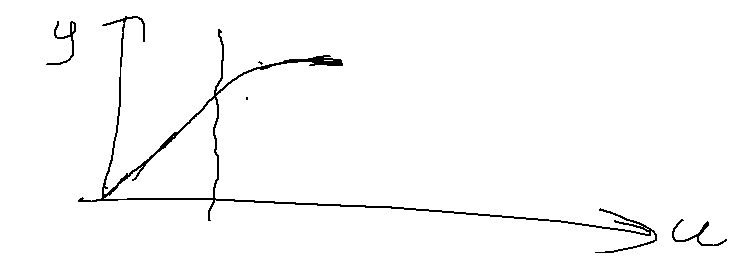
\includegraphics[width=.4\linewidth]{lec3/02_amplifier}

    Передаточная функция $ H(p) = K $.
    Чему равна весовая функция (обратное преобразование от $ H(p) $)?
    Воспользуемся

	\[ H(p) = K \Rightarrow h(t) = K \delta(t) \]

	\item \textbf{Дифференцирующее звено:}
    \[ \xrightarrow{u} \boxed{H(p)=p} \xrightarrow{y} \]
    $ m=1, n=0 $. Это нереализуемое звено! (формально).
	Зачем же оно нужно, если реализовать его нельзя?
	Полезно в связи с другими.
    Например, пусть передаточная функция такая:
    \[ H(p) = \frac{p}{T^2 p^2 + 1} \]

    Можно представить как последовательное соединение двух звеньев:

    \[ \to \boxed{p} \to \boxed{\frac{1}{T^2 p^2 + 1}} \]

    Почему <<дифференцирующее>>?
    \[ \bar y = H \bar u = p \bar u \Rightarrow y = \dot u \]

    Весовая функция есть отклик на дельта-функцию: $ h(t) = \dot \delta(t) $

    Как брать производную от дельта-функции?
    Рассмотрим $ \tilde 1[t] $ -- функцию, сшитую из двух парабол, которая в пределе стремится к функции Хевисайда.
    Возьмём её производную $ \tilde \delta(t) $.
    Это кусочно-линейная функция, у неё существует производная.

    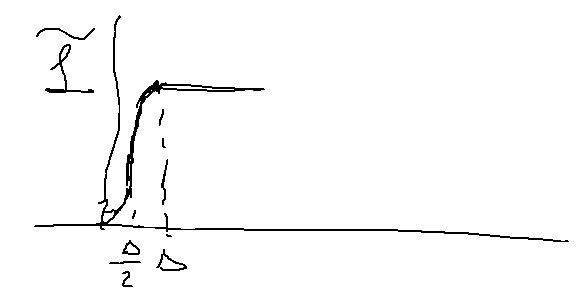
\includegraphics[width=.3\linewidth]{lec3/04_pseudo_heaviside2}
    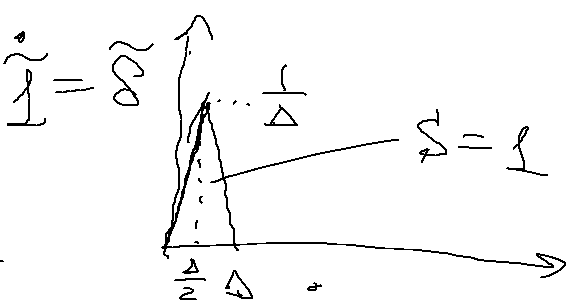
\includegraphics[width=.3\linewidth]{lec3/05_pseudo_delta}

    Производная $ \dot{ \tilde \delta }(t) $ -- два узких и высоких импульса.

    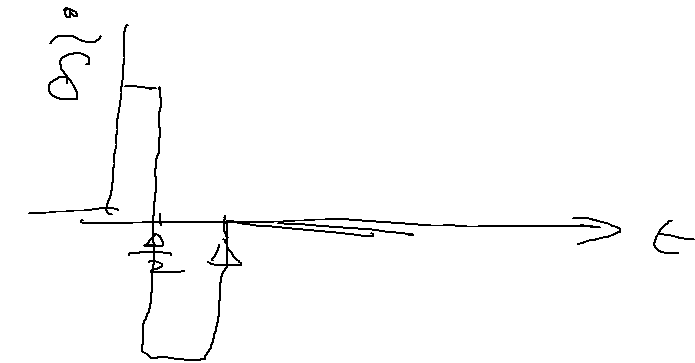
\includegraphics[width=.3\linewidth]{lec3/06_pseudo_delta_derivative}


	Т. о. производная дельта-функции -- два бесконечно узких и высоких импульса, направленных в разные стороны.

	\item \textbf{Интегрирующее звено:}

    \[ \xrightarrow{\bar u} \boxed{\frac{1}{p}}\xrightarrow{\bar y} \]

    \begin{leftbar}
        Ещё одно свойство преобразования Лапласа, которое забыли написать раньше:
        \[ \mathds{L}\left\{ \int_{0}^{t} f(\tau) d\tau \right\} = \frac{1}{p} \bar f(p) \]
    \end{leftbar}
    \[ \bar y = \frac{1}{p} \bar u \]
    \[ h(t) = 1[t] \]
    \[ y(t) = \int_{0}^{t} u(\tau) d \tau \]
\end{enumerate}

\end{document}
